\documentclass[manuscript]{aastex}
\newcommand{\vdag}{(v)^\dagger}

\usepackage{mathtools}
\usepackage{upgreek}

\newcommand{\true}{\text{true}}
\newcommand{\fit}{\text{fit}}
\newcommand{\basis}{\text{best}}
\newcommand{\rms}{\text{RMS}}
\newcommand{\dd}{\text{d}}

\shorttitle{Designing Large Scale Imaging Surveys for Retrospective Relative Photometric Calibration}
\shortauthors{Holmes et al.}

%% This is the end of the preamble.  Indicate the beginning of the
%% paper itself with \begin{document}.

\begin{document}

%% LaTeX will automatically break titles if they run longer than
%% one line. However, you may use \\ to force a line break if
%% you desire.

\title{Optimizing Large Scale Imaging Surveys for a Retrospective Relative Photometric Calibration}

%% Use \author, \affil, and the \and command to format
%% author and affiliation information.
%% Note that \email has replaced the old \authoremail command
%% from AASTeX v4.0. You can use \email to mark an email address
%% anywhere in the paper, not just in the front matter.
%% As in the title, use \\ to force line breaks.

\author{Rory Holmes, David W. Hogg\altaffilmark{1} and Hans-Walter Rix}
\affil{Max-Planck-Institut f\"ur Astronomie, K\"onigstuhl 17, Heidelberg, 69117, Germany.}
\altaffiltext{1}{2 Center for Cosmology and Particle Physics, Department of Physics, New York University, 4 Washington Place, New York, NY 10003, USA.}


\begin{abstract}
In this paper we show that, with a well chosen observing strategy, it is possible to accurately calibrate instruments used in large-scale imaging surveys with survey science data alone. We create end-to-end simulations of an imaging survey, which produces simulated datasets from mock observations of a synthetic sky according to a defined survey strategy. These catalog based simulations include realistic measurement uncertainties and a complex, position-dependent instrument response. We then use a self-calibration technique to recover the relative instrument response by fitting an model that best explains the survey dataset, based on the multiple observations of (non-varying) sources at different focal plane positions. By considering four simple survey strategies we find that, with appropriate redundancy built into the survey strategy, it is possible to accurately constrain the relative photometric response of an imaging instrument, and therefore the relative calibration of all the images and the relative fluxes of all the sources observed. The majority of the remaining post-self-calibration errors are due to the limitations in the basis used to model the relative instrument response. We find that returning the same sources to very different focal plane positions is the key property of any survey strategy designed for accurate calibration. The results of this work suggest the following advice for those considering the design of large scale imaging surveys: Do not use a regular tiling of the sky; instead return the same sources to very different focal plane positions.
\end{abstract}

\keywords{Relative Photometric Calibration: Imaging Survey: Survey Strategy}

\section{Introduction}
Astronomers tend to think in terms of taking science data and calibration data separately. The former is used for scientific measurements of astronomical sources and the latter is used to constrain instrument parameters, such as the instrument response, the dark currents and so-on. But typically far more photons, or readout electrons, are collected during science exposures themselves; are these not incredibly constraining on the calibration? Indeed, in the retrospective photometric calibration of the Sloan Digital Sky Survey data (SDSS), much more calibration information was obtained from the science data than the calibration data \citep{pad08}. But, of course, the SDSS imaging strategy had to be adjusted to make this calibration work: Good redundancy is required in the data stream, and a redundancy of a very specific kind.

In this paper, we argue that the next generation of large-scale imaging surveys should have their observation strategies designed from the very start with this kind of ``self-calibration'' in mind. This work focuses on the relative photometric calibration of a typical imaging instrument only, although similar techniques could be used to constrain many other calibration parameters, such as the optical distortion, point-spread-functions and so-on. The self-calibration technique utilizes the multiple measurements of (non-varying) sources, at different focal plane positions and at different times within the survey, to constrain the relative instrument response by requiring that the post-calibration measurements yield consistent flux values. Through end-to-end, catalog-level survey simulations, we aim to identify the important properties of survey strategies that makes them advantageous for this kind of self-calibration. 

We construct realistic survey datasets through mock observations of a synthetic sky according to a specified survey strategy. These simulations include a complex, position-dependent instrument response for the imaging instrument. Through the self-calibration procedure, we recover this instrument response by fitting a model that best describes the survey dataset. By comparing the \textit{fitted} instrument response to the \textit{true} instrument response we are able to assess the performance of the self-calibration procedure with different survey strategies. There is a degeneracy in this problem: the self-calibration procedure is only able to fit for a \textit{relative} instrument response. We have no way to know, for example, if all the sources are uniformly fainter, or if the instrument sensitivity is uniformly lower. 

In this work we do not produced pixelated images; instead we concentrate on catalog-level simulations with realistic measurement uncertainties. Complex effects are included in the simulations that are not  precisely modeled at the analysis stage, in order to simulate the effects of unknown systematic errors within the dataset.

In Section \ref{sec:survey_simulations} we introduce the simulation chain constructed to produce the realistic survey datasets. Section \ref{sec:self_cal} goes onto to detail the self-calibration procedure, with Section \ref{sec:metrics} summarizing the metrics we use to assess its performance. In Section \ref{sec:simple_surveys} we focus on four simple survey strategies, which allow us to draw conclusions on the performance of the self-calibration procedure with different survey properties. 

\section{Survey Dataset Simulations}
\label{sec:survey_simulations}
We have constructed an end-to-end simulation chain that produces a realistic imaging dataset from a specified survey strategy. In this work we have kept the simulation parameters intentionally flexible, so that the sensitivity of the self-calibration procedure to different values can be investigated. The simulations are split into a number of steps. The first is the generation of a synthetic sky. With a given pointing, single mock observations are performed on this sky. To build up a full-survey dataset, multiple single observations are performed according to the specified survey strategy. In this section, we detail the assumptions and methods used in each of these steps. 

\subsection{The Synthetic Sky}
We generate a representative synthetic sky based on realistic object densities in the AB magnitude range $m_\text{min} = 17$ to $m_\text{max} = 22$~mag$_\text{AB}$, with these limits chosen to be consistent with the saturation and $10\upsigma{}$ limits of deep, space-based, near-infrared survey. Sources are generated with random coordinates (uniformly distributed within the sky region being investigated) and with random magnitudes $m$ distributed according to
\begin{eqnarray}
\log_{10} \frac{\dd N}{\dd m \, \dd \Omega} = a + b\,m + c\,m^2 \label{eqn:power_law} \quad , 
\end{eqnarray}
where $\dfrac{\dd N}{\dd m \, \dd  \Omega}$  is the density of sources $N$ per unit magnitude $m$ and per unit solid angle $\Omega$, and $a$, $b$ and $c$ are model parameters. Even though our simulations make no distinction between galaxies and stars, the values of the parameters are found from fitting the Y-band galaxy populations reported in \citet{win11} only. These parameters were found to be $a = -13.05$, $b = 1.25$ and $c = -0.02$. The source magnitudes $m$ are related to the source fluxes $s$ simply by: $m = 22.5 - 2.5\log_{10}(s)$, where the 22.5 puts the fluxes in units of nanomaggies (nmgy). To limit the data, we only select the brightest sources within the survey area, up to a source density per unit solid angle $d$, for the self-calibration procedure.

\subsection{A Single Exposure}
\label{sec:single_exposure}
With a camera pointing $(\alpha, \beta)$ and camera orientation $\theta$ this synthetic sky is transformed into focal plane image. In our simulations, we use a large instrument field-of-view of $0.76~ \text{deg} \times 0.72~\text{deg}$; a size consistent with the next generation of large survey imagers. An example of a single pointing exposure is shown in Figure \ref{fig:single_image}.

\subsubsection{Measured Count Rates}
We do not consider pixelated images in these simulations; instead the true source fluxes $s_\true$ are converted into measured count rates $c$ with an complex, position-dependent instrument response model $f_\true$ and a measurement noise model. For a measurement $i$ the count rate $c_i$ recorded from a source $k$ depends on the \textit{true} instrument response $f_{\true}(\vec{x_i} | \vec{q}_\true)$, which is a function of focal plane position $\vec{x_i}$, and the source's true flux $s_{k,\true}$ 
\begin{eqnarray*}
c_i = f_{\true}(\vec{x_i} | \vec{q}_\true) \, s_{k, \true} + e_{i} \quad ,
\end{eqnarray*}
where $\vec{q}_\true$ are the parameters defining the \textit{true} instrument response, and $e_i$ is a noise contribution drawn from the Normal Distribution $N(e|0,{\sigma_\true}^2)$. 

\subsubsection{Noise Model}
\label{sec:noise}
To construct the noise model, the simulated exposures are assumed to be background limited and that, for systematic reasons, there is an upper limit on the signal-to-noise ratio of 500 for bright sources. The noise model is complicated further by applying an extra term $\epsilon_i$ to the count rates' uncertainty variance, which we intentionally do not take into account in the analysis in order to simulate systematic problems with the instrument noise model. The \textit{true} noise model is therefore
\begin{eqnarray}
\sigma_{i, \true}^{2} = (1 + \epsilon_i) \, \alpha^{2} + \eta^{2}\, [ f_\true(\vec{x_i} | \vec{q}_\true) \, s_{k, \true} ]^2 \quad , \label{eqn:noise}
\end{eqnarray}
where $\alpha$ and $\eta$ are both constants and $\epsilon_i$ is a random number, drawn uniformly in the range [0.0, $\epsilon_{max}$), generated for each measurement $i$. The $m = 22$ mag 10$\upsigma$ detection limit introduced previously and the 500 limit on the signal-to-noise ratio are used to set $\alpha = 0.1585$ and $\eta = 0.0017$. The $\epsilon_i$ contribution is not taken into account in the analysis and therefore the uncertainty variances on the count rates are \textit{assumed} (incorrectly, but realistically) to be
\begin{eqnarray*}
\sigma_{{i}}^{2} = \alpha^{2} + \eta^{2} \, c^{2}_i \quad 
\end{eqnarray*}
during this stage. 

\subsubsection{The True Instrument Response Model}
\label{sec:instrument_response_model}
We construct a complex, position independent instrument response model $f_\true(\vec{x_i} | \vec{q}_{\true})$ from a superposition of large and small-scale variations:
\begin{eqnarray*}
f_\true(\vec{x_i} | \vec{q}_{\true, 1 \ldots 260}) = f_\text{large}(\vec{x_i} | \vec{q}_{\true, 1 \ldots 6}) + f_\text{small}(\vec{x_i} | \vec{q}_{\true, 7 \ldots 260}) \quad ,
\end{eqnarray*}
where $\vec{x_i} = (x_i, y_i)$ is the focal plane position that the $k$th source falls at during the $i^\text{th}$ measurement and $\vec{q}_\true$ are the parameters defining the instrument response model. The large-scale instrument response $f_\text{large}(\vec{x_i} | \vec{q}_{\true, 1 \ldots 6})$ is modeled as a second order polynomial:
\begin{eqnarray*}
f_\text{large}(\vec{x_i} | \vec{q}_{\true, 1 \ldots 6}) = q_{\true, 1} + q_{\true, 2} \, x_i + q_{\true, 3} \, y_i + q_{\true, 4} \, x_i^2 + q_{\true, 5} \, x_i \, y_i  + q_{\true, 6} \, y_i^2  \quad .
\end{eqnarray*}
The small-scale instrument response, which is constructed from sine and cosine contributions, is superimposed on this large-scale instrument response. The small-scale instrument response $f_\text{small}(\vec{x_i} | \vec{q}_{\true, 7 \ldots 260})$ is modeled as
\begin{eqnarray*}
f_\text{small}(\vec{x_i} | \vec{q}_{\true, 7\ldots 260})  & = &  \sum_{a=0}^6 \sum_{b=0}^a \left[ q_{\true, 7+4b} \cos (k_x \, x_i) + q_{\true, 8+4b} \sin (k_x \, x_i) \right] \\
& & \qquad \qquad \times \left[ q_{\true, 9+4b} \cos (k_y \, y_i) + q_{\true, 10+4b} \sin (k_y \, y_i) \right] \quad ,
\end{eqnarray*}
where
\begin{eqnarray*}
k_x & = & \dfrac{a \, \pi}{X} \quad ,\\
k_y & = & \dfrac{b \, \pi}{Y} \quad ,\\
\end{eqnarray*}
with the physical focal plane dimensions $X$ and $Y$. In total, the instrument response model is parameterized with 260 parameters; an example can be seen in Figure \ref{fig:single_image}      (right). It is this instrument response that we try and recover with the self-calibration procedure. Our final assumption in these simulations is that the instrument response is temporally stable. 

\subsection{The Complete Survey}
In this work we are interested in simulating complete surveys, in order to identify the crucial characteristics of survey strategies that allow for the relative instrument response model to be accurately, retrospectively constrained from the resulting dataset. We therefore apply the single exposure procedure introduced in the previous section for each pointing specified in a defined survey strategy. The resultant source measurements are collated into a survey-wide dataset. 

\section{Self-Calibrating the Survey-Wide Dataset}
\label{sec:self_cal}
We self-calibrate the dataset generated in the survey simulations to recover a best possible estimate of the true instrument response applied and the true source fluxes. This self-calibration procedure has been successfully applied to ground-based imaging surveys, such as the Sloan Digital Sky Survey \citep{pad08}\footnote{Here this procedure is dubbed ``uber-calibration.''}. This iterative procedure comprises two steps: (1) a refinement of the source flux estimates based on the latest instrument response model and (2) a refinement of the instrument response model based on the updated source flux estimates. These steps are iterated until the system converges, or until it is clear that the system will not converge. There is a degeneracy in the problem, as both the true instrument response and the true source magnitudes are unknown. It is therefore only possible to calibrate the \textit{relative} instrument response and the \textit{relative} source fluxes. It is not possible to know, for example, if the sources are all fainter or if the instrument response is uniformly lower. In practice, this degeneracy can be broken through observations of a small number of standard absolute sources.

\subsection{Fitted Measurement Model}
To complicate the simulations, we use the self-calibration procedure to fit a model that is \textit{incomplete} in two ways. Firstly, the \textit{fitted} instrument response is modeled as an eighth order polynomial, and not the second order polynomial superimposed with sine and cosine contributions used to model the \textit{true} instrument response. Secondly, the assumed measurement uncertainty variances do not include the additional random measurement error $\epsilon_{i}$ introduced in Subsection \ref{sec:noise}. The incomplete measurement model is
\begin{eqnarray*}
c_i = f(\vec{x_i} | \vec{q}) \, s_{k} + e_{i} \quad ,
\end{eqnarray*}
where $c_i$ is the recorded count rate, $f(\vec{x_i} | \vec{q})$ is the fitted instrument response model at a focal plane position $\vec{x}_i$, $\vec{q}$ is a vector parameterizing the eighth order polynomial instrument response model, $s_k$ is the model source flux estimate and the error $e_i$ is drawn from the Normal Distribution $N(e|0,{\sigma_i}^2)$, such that
\begin{eqnarray*}
\sigma_{{i}}^{2} = \alpha^{2} + \eta^{2}\, c^{2}_i \quad ,
\end{eqnarray*} 
where $\alpha$ and $\eta$ are the parameters set by the instruments $10\upsigma$ and saturation limits. The $\epsilon_i$ error contribution is intentionally not included in order to simulate systematic problems with the instrument noise model. 

We make one further assumption during this analysis phase: We assume that clearly variable sources have been removed from the source catalog, and that the remaining sources vary by less than $\epsilon_{max}$.

\subsection{Step 1: Source Flux Refinement}
The sources are considered individually in the first step of the self-calibration procedure; their flux estimates are refined based on the latest fitted instrument response parameters $\vec{q}$. An error function $\chi^2_{k}$ for all the measurements $i$ of a source $k$ ($i \in \mathcal{O}(k)$) is constructed:
\begin{eqnarray*}
\chi^2_{k} = \sum_{i \in \mathcal{O}(k)} \frac{(c_i-f_{i}(\vec{x_i} | \vec{q}) \, s_{k})^2}{{\sigma_i}^2} \quad ,
\end{eqnarray*}
where $c_i$ are the measured count rates, $f(\vec{x_i} | \vec{q})$ is the fitted instrument response model at a focal plane position $\vec{x}_i$ and $\sigma_i$ is the assumed noise model. A new estimate of the model source flux $s'_{k}$ is then found by minimizing the error function with respect to the old model source flux $s_{k}$:
\begin{eqnarray*}
\frac{d\chi^2_{k}}{d s_{k}} = \sum_{i \in \mathcal{O}(k)} \frac{-2 f_{i}(\vec{x_i} | \vec{q}) \, (c_i-f_{i}(\vec{x_i} | \vec{q}) \, s'_{k})}{{\sigma_i}^2} = 0 \quad ,
\end{eqnarray*}
\begin{eqnarray*}
s'_{k} \leftarrow \left[{\sum_{i \in \mathcal{O}(k)}  \frac{f_{i}(\vec{x_i} | \vec{q})^2}{{\sigma_i}^2}} \right]^{-1}  \left[ {\sum_{i \in \mathcal{O}(k)} \frac{f_{i}(\vec{x_i} | \vec{q}) \, c_i}{{\sigma_i}^2}} \right] \quad .
\end{eqnarray*}
The standard uncertainty variance on the new source flux estimate $s'_{k}$ is given by
\begin{eqnarray*}
\sigma'^2_k = \left[{\sum_{i \in \mathcal{O}(k)}  \frac{f_{i}(\vec{x_i} | \vec{q})^2}{{\sigma_i}^2}} \right] \quad .
\end{eqnarray*}


\subsection{Step 2: Instrument Response Refinement}
The instrument response parameters can now be refined with the latest source flux estimates. A error function for all the measurements of all the sources is constructed
\begin{eqnarray*}
\chi^2 = \sum_{k} \chi'^2_k \quad ,
\end{eqnarray*}
where
\begin{eqnarray*}
\chi'^2_k = \sum_{i \in \mathcal{O}(k)} \frac{(c_i-f_{i}(\vec{x_i} | \vec{q}) \, s'_{k})^2}{{\sigma_i}^2}  \quad .
\end{eqnarray*}
Recall that the fitted instrument response $f_{i}(\vec{x_i} | \vec{q})$ is modeled as an eighth order polynomial. This can be expressed as
\begin{eqnarray*}
f_{i}(\vec{x_i} | \vec{q}) = \sum_{l = 1}^L q_{l} \, g_l(\vec{x_i})  \quad ,
\end{eqnarray*}
where $L = 45$ in this case. The total error function $\chi^2$ can be rewritten as
\begin{eqnarray*}
\chi^2 =\sum_{k} \sum_{i \in \mathcal{O}(k)} \frac{(c_i- s'_{k} \sum_{l = 1}^L q_{l} g_l(\vec{x_i}))^2}{{\sigma_i}^2}   \quad .
\end{eqnarray*}
To refine the instrument response model fit, this error function is minimized with respect to the instrument response model parameters $q_{l}$
\begin{eqnarray*}
\frac{d\chi^2}{dq_{l}} = \sum_{k} \sum_{i \in \mathcal{O}(k)} \frac{-2 g_l(\vec{x_i}) s'_{k} (c_i- s'_{k} \sum_{l' = 1}^{L'} q'_{l'} g_{l'}(\vec{x_i}))}{{\sigma_i}^2} = 0  \quad ,
\end{eqnarray*}
\begin{eqnarray*}
\sum_{k} \sum_{i \in \mathcal{O}(k)} \frac{g_l(\vec{x_i}) s'_{k} c_i}{{\sigma_i}^2} = \sum_{k} \sum_{i \in \mathcal{O}(k)} \frac{g_l (\vec{x_i}) s'^2_{k} \sum_{l' = 1}^{L'} q'_{l'} g_{l'} (\vec{x_i})} {{\sigma_i}^2}   \quad .
\end{eqnarray*}
It is now simpler to proceed in matrix notation. The following substitutions can be made
\begin{eqnarray}
b_l & = & \sum_{k} \sum_{i \in \mathcal{O}(k)} \frac{g_l(\vec{x_i}) s'_{k} c_i}{\sigma_i^2}    \quad ,\\
G_{ll'} & = & \sum_{k} \sum_{i \in \mathcal{O}(k)} \frac{{s'}_{k}^2}{\sigma_i^2} g_l(x_i) g_{l'}(x_i)   \quad .
\end{eqnarray}
The matrix equation is then
\begin{eqnarray*}
\vec{b} = G \cdot \vec{q'}    \quad .
\end{eqnarray*}
The refined instrument response parameters are then found by
\begin{eqnarray*}
\vec{q'} \leftarrow G^{-1}  \cdot \vec{b}   \quad .
\end{eqnarray*}
These two steps are iterated until the solution converges to a final fit of the instrument response $f_\fit(\vec{x} | \vec{q_\fit})$ and the source fluxes $s_{k,\fit}$, or until it is clear that a solution will not be found. 

\section{Metrics}
\label{sec:metrics}
To assess the performance of the self-calibration procedure with different survey strategies, it is necessary to quantify the quality of the final fitted solution. To do this we defined three quantities. The first is the root-mean-squared (RMS) error $S_\text{RMS}$ in the final fitted source fluxes $s_{k,\fit}$ compared to the true source fluxes $s_{k,\true}$ for the $K$ sources used in the self-calibration procedure:
\begin{equation}
S_\text{RMS} = \sqrt{\dfrac{1}{K} \sum_k^K \left( \dfrac{s_{k,\fit} - s_{k,\true}}{s_{k,\true}} \right)^2}   \quad .
\end{equation}
The other two metrics, called ``badnesses'', are defined as the RMS error between the final fitted instrument response and a reference instrument response sampled on a regular $300 \times 300$ grid across the focal plane. For the ``true badness'' $B_\true$, the \textit{fitted} instrument response $f_\fit(\vec{x} | \vec{q_\fit})$ is compared to the \textit{true} instrument response $f_\true(\vec{x} | \vec{q_\true})$ at the $J$ sample points  
\begin{equation}
B_\true = \sqrt{\dfrac{1}{J} \sum_j^J \left(\dfrac{f_\fit(\vec{x_j} | \vec{q_\fit}) - f_\true(\vec{x_j} | \vec{q_\true})}{f_\true(\vec{x_j} | \vec{q_\true})}\right)^2}   \quad .
\end{equation}
The ``best-in-basis badness'' $B_\basis$ compares the \textit{fitted} instrument response $f_\fit(\vec{x_j} | \vec{q_\fit})$ to the \textit{best instrument response fit possible} $f_\basis(\vec{x_j} | \vec{q_\basis})$ with the basis used to describe the fitted model (in this case an eight order polynomial) at the $J$ sample points
\begin{equation}
B_\basis = \sqrt{\dfrac{1}{J} \sum_j^J \left( \dfrac{f_\fit(\vec{x_j} | \vec{q_\fit}) - f_\basis(\vec{x_j} | \vec{q_\basis})}{f_\basis(\vec{x_j} | \vec{q_\basis})} \right)^2}   \quad .
\end{equation}
The best-in-basis badness is always smaller than the true badness, as it does not include the errors associated with the limitation of the basis used for the fitted model. The badnesses provide a more complete description of the self-calibration performance than the RMS error on the fitted sources' fluxes, as the RMS source error only applies to the bright sources within the survey selected for the self-calibration procedure.

\section{Simple Survey Strategies}
\label{sec:simple_surveys}
In this paper, we consider four simple but very different survey strategies. We use the end-to-end dataset simulation and self-calibration chain, introduced in Sections \ref{sec:survey_simulations} and \ref{sec:self_cal}, to evaluate the performance of the self-calibration procedure with these strategies. 

\subsection{Survey Description}
We label the four survey strategies -- which all cover the same patch of sky -- with the letters A to D. These survey strategies are summarized in Table \ref{tab:simple_surveys} and are shown in Figure \ref{fig:simple_surveys}. Strategy A is the simplest strategy; the field is regularly tiled with small overlaps between adjacent pointings ($\sim 5$~\% and $\sim 8$~\% in the camera pointing directions $\alpha$ and $\beta$ respectively). The pointings in the 12 passes over the same field are exactly aligned. Survey B is the same as A, but with each pass over the field the orientation of the telescope is rotated by $30^\circ$. Survey C is more complex. The first pass over the field is the same as in Survey A, with $12 \times 12$ pointings. In the next pass, one of the pointings in the $\alpha$ direction is removed and one is added in the $\beta$ and the pointings are respaced uniformly, so the resultant pointing grid is $13 \times 11$. In the third pass over the field this change is reversed and the field is measured on a $11 \times 13$ grid. These three passes are then repeated four times. The pointing positions in Survey D are quasi-random: the pointings are the same as with Survey A, but each has a random offset within [-0.35,0.35)~deg applied in both the $\alpha$ and $\beta$ directions. By fixing the pointings within these $0.7~\text{deg} \times 0.7~\text{deg}$ boxes, we ensure that the quasi random strategy has a uniform coverage of the field. The orientations of the pointings in Survey D are completely random.

\subsection{Self-Calibration Performance}
The iterative self-calibration procedure converges to a final fitted solution for the Survey B, C and D datasets. With the Survey A dataset it does not converge in any reasonable time period, even when the system is started close to the optimum fit. The fitted instrument response solutions from the Surveys A to D datasets are shown in Figures \ref{fig:A_result} to \ref{fig:D_result}. In these plots the final fitted instrument response $f_\fit(\vec{x_j} | \vec{q_\fit})$ is compared to the true instrument response $f_\true(\vec{x} | \vec{q_\true})$ and to the best possible instrument response fit with the basis used $f_\basis(\vec{x_j} | \vec{q_\basis})$ (``best-in-basis''). The accuracy of the final fitted solutions are summarized, with the metrics introduced in Section \ref{sec:metrics}, for each of the Survey strategies in Table \ref{tab:simple_results}. 

The self-calibration procedure performs best with the Survey D dataset, followed by the Survey C dataset, then the Survey B dataset. The self-calibration procedure failed completely with the Survey A dataset and no solution was obtained. The number of iterations of the self-calibration procedure required to converge to the final solution also decreases as the quality of the final fit increases: Survey D required 9 iterations, Survey C 26, Survey B 4160 and the procedure was iterated 8192 times with Survey A without reaching a solution.

With the Survey C and D datasets, the instrument response is accurately recovered. As can be seen from Figures \ref{fig:C_result} and \ref{fig:D_result} (top) the fitted instrument response $f_\fit(\vec{x_j} | \vec{q_\fit})$ does not perfectly reproduce the true instrument response $f_\true(\vec{x} | \vec{q_\true})$, with residuals up to the $\pm 1~\%$ level. That said, through comparisons with the best fit possible with the eight order polynomial basis used in the self-calibration procedure $f_\basis(\vec{x_j} | \vec{q_\basis})$ (bottom), we find that majority of the remaining errors in our fits are due to limitations in the model basis used. The residuals in this comparison are low; this can also be clearly seen in the factor of $\sim 10$ improvement in the best-in-basis badness $B_\basis$ compared to the true badness $B_\true$. The results from these two survey datasets are clear: if the correct redundancy is built into the survey, then self-calibration calibration can be used to accurately constrain the relative instrument response, with presumably the majority of the remaining errors coming from the limitations in the model used to represent the instrument response.

The Survey A and B datasets also give interesting results. With Survey A, the self-calibration procedure did not reach a solution. This -- in itself -- is an important result, as the naive tiling of the sky currently being considered for many large surveys will result in datasets that cannot be retrospectively self-calibrated. Minor changes to survey strategies, such as those in Survey C, can drastically improve the performance of the self-calibration procedure. Without these changes, vast amounts of calibration information is simply lost. We can also draw conclusions from the results obtained with Survey B: here the self-calibration procedure converges close to the correct solutions, albeit not as close as the Surveys C and D. Here, it is the quality of the fit over the focal plane that is interesting. From the residual plot against the best-in-basis instrument response $f_\basis(\vec{x_j} | \vec{q_\basis})$ (Fig \ref{fig:B_result} bottom right), we can see that the quality of the fit is rotationally symmetric, with the self-calibration procedure able to fit the instrument response well at the edge of the focal plane, but poorly at the center. 

This, along with the success of the procedure with the Surveys C and D datasets, gives an insight into the key property of a survey that makes it good for self-calibration. Namely, the survey should return the same sources to many, very different focal plane positions. This allows the self-calibration procedure to link the different parts of the focal plane with each other through the observations of the same sources. Surveys C and D do this, and the self-calibration procedure performs well with their dataset. Survey A does not do this; it only connects the outer edges of the focal plane to each other. There are no redundant measurements connecting the majority of the focal plane to other positions. This conclusion in confirmed with Strategy B. Here, positions at the outside of the focal plane are well connected to other positions and therefore the self-calibration procedure can well fit the instrument response in these regions. In the center of the focal plane, on which the same sources always fall, there are insufficient redundant measurements to allow for a good fit. Returning the same sources to very different focal plane positions is critical for the self-calibration to work effectively. 

\section{Discussion}
From the simulations presented in this paper, we are draw two firm conclusions about the self-calibration of large-scale imaging surveys. The first is that, in agreement with previous work, we show that this technique is very powerful, allowing the relative instrument response of an imaging instrument to be accurately retrospectively constrained from the science images alone. The second is that there must be the correct redundancy built into the survey strategy. The same sources must be imaged at very different focal plane positions; regular tiling of the sky is useless for this kind of calibration. 

In this paper, we have considered the design of survey strategies for calibrating the relative photometric response of an instrument, but we feel there are many more calibration parameters that can be constrained from this method. For example, the optical distortion of an instrument or the point-spread-function variation could also be constrained with such a method, although we concede that the properties of a survey strategy that makes them good for one calibration, may not be the same as that for another; ultimately a trade-off would need to be performed between the different calibration concerns and the other goals of the survey, such as sky coverage, variability monitoring and so-on. 

All of the code used in this work is publicly available at XX.

\acknowledgments
\section{Acknowledgments}
We are grateful to 

\appendix

%% The reference list follows the main body and any appendices.
%% Use LaTeX's thebibliography environment to mark up your reference list.
%% Note \begin{thebibliography} is followed by an empty set of
%% curly braces.  If you forget this, LaTeX will generate the error
%% "Perhaps a missing \item?".
%%
%% thebibliography produces citations in the text using \bibitem-\cite
%% cross-referencing. Each reference is preceded by a
%% \bibitem command that defines in curly braces the KEY that corresponds
%% to the KEY in the \cite commands (see the first section above).
%% Make sure that you provide a unique KEY for every \bibitem or else the
%% paper will not LaTeX. The square brackets should contain
%% the citation text that LaTeX will insert in
%% place of the \cite commands.

%% We have used macros to produce journal name abbreviations.
%% AASTeX provides a number of these for the more frequently-cited journals.
%% See the Author Guide for a list of them.

%% Note that the style of the \bibitem labels (in []) is slightly
%% different from previous examples.  The natbib system solves a host
%% of citation expression problems, but it is necessary to clearly
%% delimit the year from the author name used in the citation.
%% See the natbib documentation for more details and options.

\begin{thebibliography}{}
\bibitem[Padmanabhan et al. (2008)]{pad08} {Padmanabhan, N. et al., An Improved Photometric Calibration of the Sloan Digital Sky Survey Imaging Data, 2008, \apj, 674, 1217}
303	\bibitem[Windhorst et al. (2011)]{win11}{Windhorst, R.~A. et al., The Hubble Space Telescope Wide Field Camera 3 Early Release Science Data: Panchromatic Faint Object Counts for 0.2-2 $\upmu$m Wavelength, 2011, XX.}
\end{thebibliography}
\clearpage



%% Use the figure environment and \plotone or \plottwo to include
%% figures and captions in your electronic submission.
%% To embed the sample graphics in
%% the file, uncomment the \plotone, \plottwo, and
%% \includegraphics commands
%%
%% If you need a layout that cannot be achieved with \plotone or
%% \plottwo, you can invoke the graphicx package directly with the
%% \includegraphics command or use \plotfiddle. For more information,
%% please see the tutorial on "Using Electronic Art with AASTeX" in the
%% documentation section at the AASTeX Web site, http://aastex.aas.org/
%%
%% The examples below also include sample markup for submission of
%% supplemental electronic materials. As always, be sure to check
%% the instructions to authors for the journal you are submitting to
%% for specific submissions guidelines as they vary from
%% journal to journal.

%% This example uses \plotone to include an EPS file scaled to
%% 80% of its natural size with \epsscale. Its caption
%% has been written to indicate that additional figure parts will be
%% available in the electronic journal.

%% Here we use \plottwo to present two versions of the same figure,
%% one in black and white for print the other in RGB color
%% for online presentation. Note that the caption indicates
%% that a color version of the figure will be available online.
%%


%% This figure uses \includegraphics to scale and rotate the still frame
%% for an mpeg animation.


%% If you are not including electonic art with your submission, you may
%% mark up your captions using the \figcaption command. See the
%% User Guide for details.
%%
%% No more than seven \figcaption commands are allowed per page,
%% so if you have more than seven captions, insert a \clearpage
%% after every seventh one.

%% Tables should be submitted one per page, so put a \clearpage before
%% each one.

%% Two options are available to the author for producing tables:  the
%% deluxetable environment provided by the AASTeX package or the LaTeX
%% table environment.  Use of deluxetable is preferred.
%%

%% Three table samples follow, two marked up in the deluxetable environment,
%% one marked up as a LaTeX table.

%% In this first example, note that the \tabletypesize{}
%% command has been used to reduce the font size of the table.
%% We also use the \rotate command to rotate the table to
%% landscape orientation since it is very wide even at the
%% reduced font size.
%%
%% Note also that the \label command needs to be placed
%% inside the \tablecaption.

%% This table also includes a table comment indicating that the full
%% version will be available in machine-readable format in the electronic
%% edition.


\begin{figure}[ht]
\begin{center}
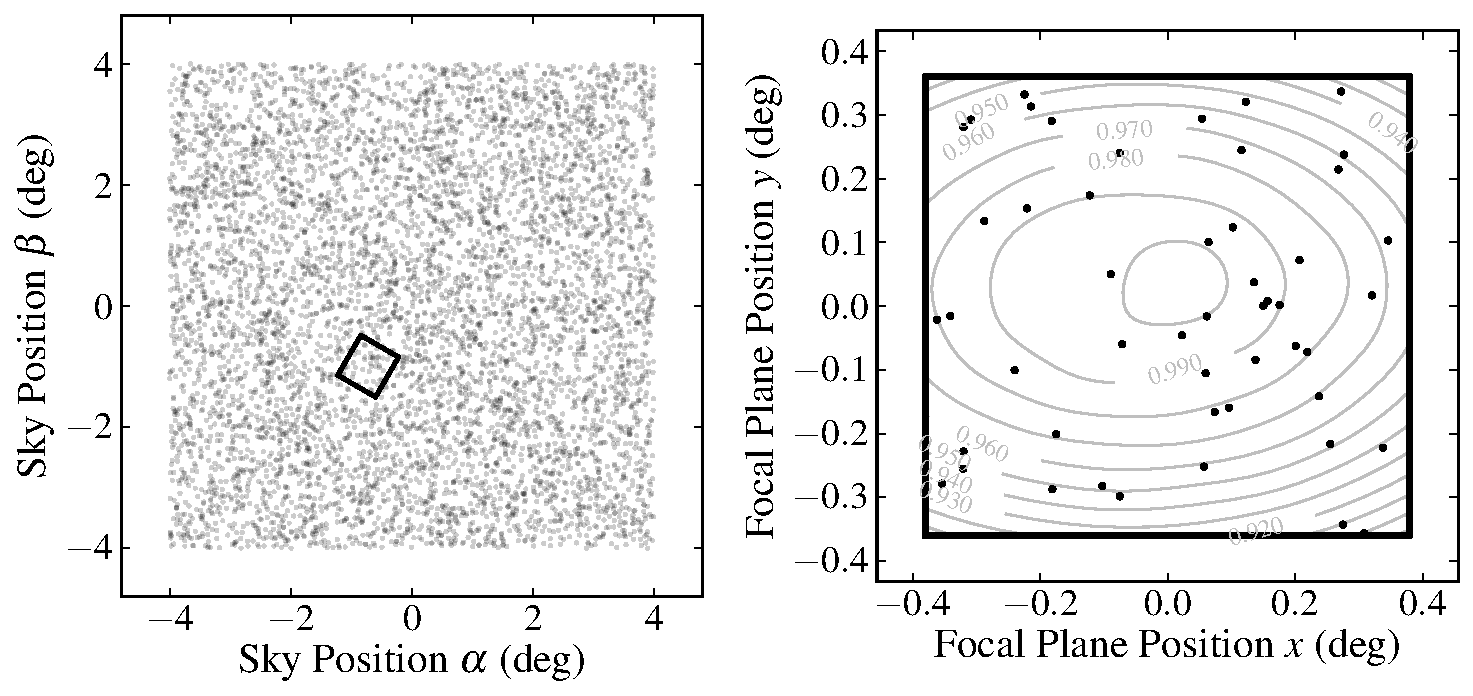
\includegraphics[width=\textwidth]{./single_image.pdf}
\end{center}
\caption{A single exposure of the synthetic sky. Left: A plot of the bright sources within the synthetic sky used in the self-calibration procedure, with the focal plane footprint overlaid. Right: The resultant distribution of the sources on the instrument's focal plane. The \textit{true} instrument model $f_{\true}(\vec{x_i} | \vec{q}_\true)$ is shown with contours.\label{fig:single_image}}
\end{figure}

\clearpage
\begin{deluxetable}{lc}
\tablewidth{0pt}
\tablecaption{A summary of the tuneable parameters in these simulations and their fiducial values.\label{tab:parameters}}
\tablehead{
\colhead{Parameter} & \colhead{Fiducial Value}}
\startdata
Source Density -- Eqn. \ref{eqn:power_law} (deg$^{-2}$) & $a=-13.05, b=1.25, c=-0.02$ \\
Survey Area (deg$^2$)& $8 \times 8$ \\
Source Density (deg$^{-2}$) & $ d = 100 $ \\
Saturation Limit (mag) & $m_\text{min} = 17$\\
10$\upsigma$ Detection Limit (mag)& $m_\text{max} = 22$\\
Field-of-View (deg$^{2}$)& $0.76 \times 0.72$ \\
Noise Model -- Eqn. \ref{eqn:noise} & $\alpha = 0.1585$, $\eta = 0.0017$, $\epsilon_\text{max} = 1.0$\\
Fitted Instrument Response Model & 8$^{\text{th}}$ order polynomial\\
\enddata
\end{deluxetable}

\clearpage
\begin{deluxetable}{cccc}
\tablewidth{0pt}
\tablecaption{A summary of the four simple survey strategies considered in this paper. \label{tab:simple_surveys}}
\tablehead{
\colhead{Survey Label} & \colhead{Pointing Center} & \colhead{Orientation} & \colhead{Number of Pointings}}
\startdata
A  & Uniform Grid ($12\times12$) & $0^\circ$ & 1728 \\
B      & Uniform Grid ($12\times12$)     & Each Pass: $\theta +30^\circ$& 1728 \\
C   & Pass 1:  Uniform Grid ($12\times12$)  &  & 1720\\
 & Pass 2:  Uniform Grid ($13§\times11$) & $0^\circ$&\\
  & Pass 3:  Uniform Grid ($11§\times13$) & &\\
D   & Quasi-Random  & Random & 1728\\
\enddata
\end{deluxetable}



\begin{figure}[ht]
\begin{center}
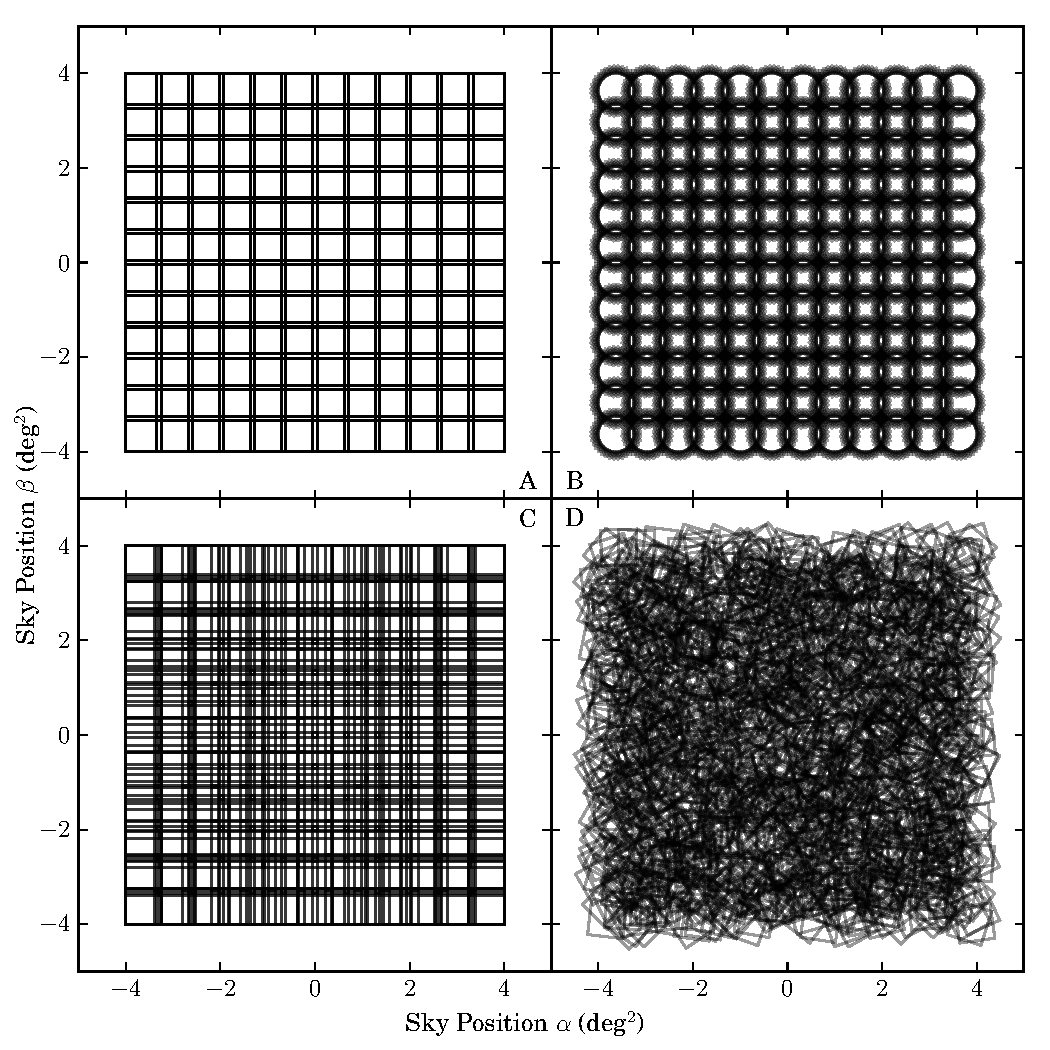
\includegraphics[width=\textwidth]{simple_surveys.pdf}
\end{center}
\caption{Focal plane footprints projected onto the synthetic sky according to the four simple survey strategies described in Section \ref{sec:simple_surveys} and summarized in Table \ref{tab:simple_surveys}. Surveys A, B and D have 1728 pointings and survey C has 1720 pointings.\label{fig:simple_surveys}}
\end{figure}

\begin{figure}[ht]
\begin{center}
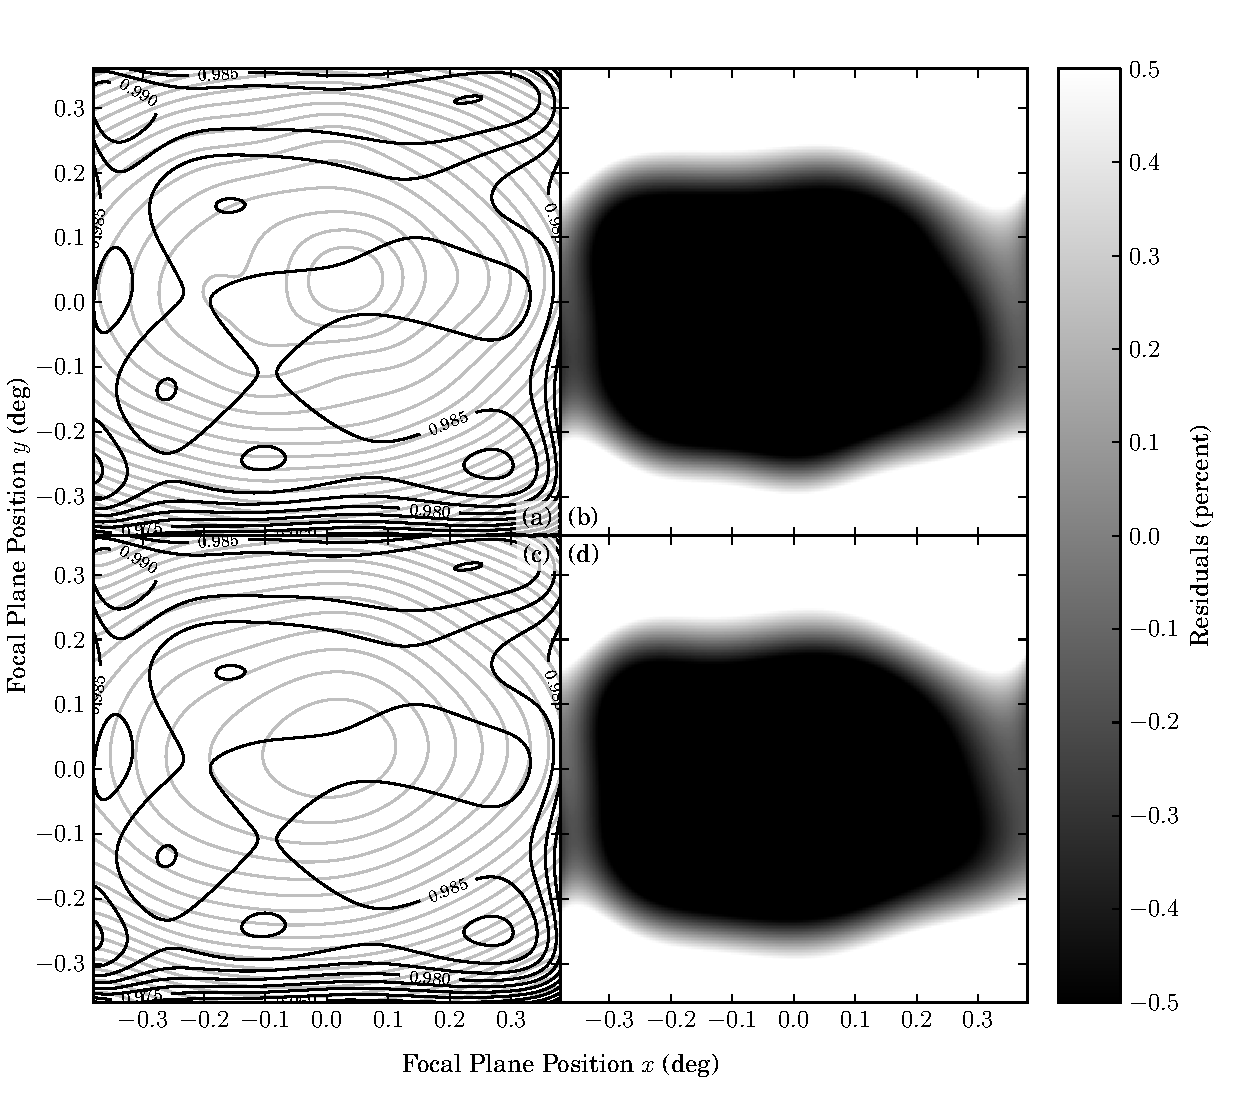
\includegraphics[width=\textwidth]{A_8192_ff.pdf}
\end{center}
\caption{A comparison of the fitted instrument response model $f_\fit(\vec{x_j} | \vec{q_\fit})$ obtained from self-calibrating the Survey A dataset compared to the true $f_\true(\vec{x} | \vec{q_\true})$ and best-in-basis $f_\basis(\vec{x_j} | \vec{q_\basis})$ instrument response models. The self-calibration procedure did not converged to the final solution and the results presented here correspond to the instrument response found after $8192$ iterations. (a) Contour plot of the fitted (black) compared to the \textit{true} (gray) instrument response. (c) Contour plot of the fitted (black) compared to the \textit{best-in-basis} (gray) instrument response model. The best-in-basis instrument response is the best fit to the true instrument response possible with the basis used to model the instrument response in the self-calibration procedure (in this case an eighth order polynomial). The plots (b) and (d) show the residuals between the two instrument response models plotted in (a) and (c) respectively.\label{fig:A_result}}
\end{figure}

\begin{figure}[ht]
\begin{center}
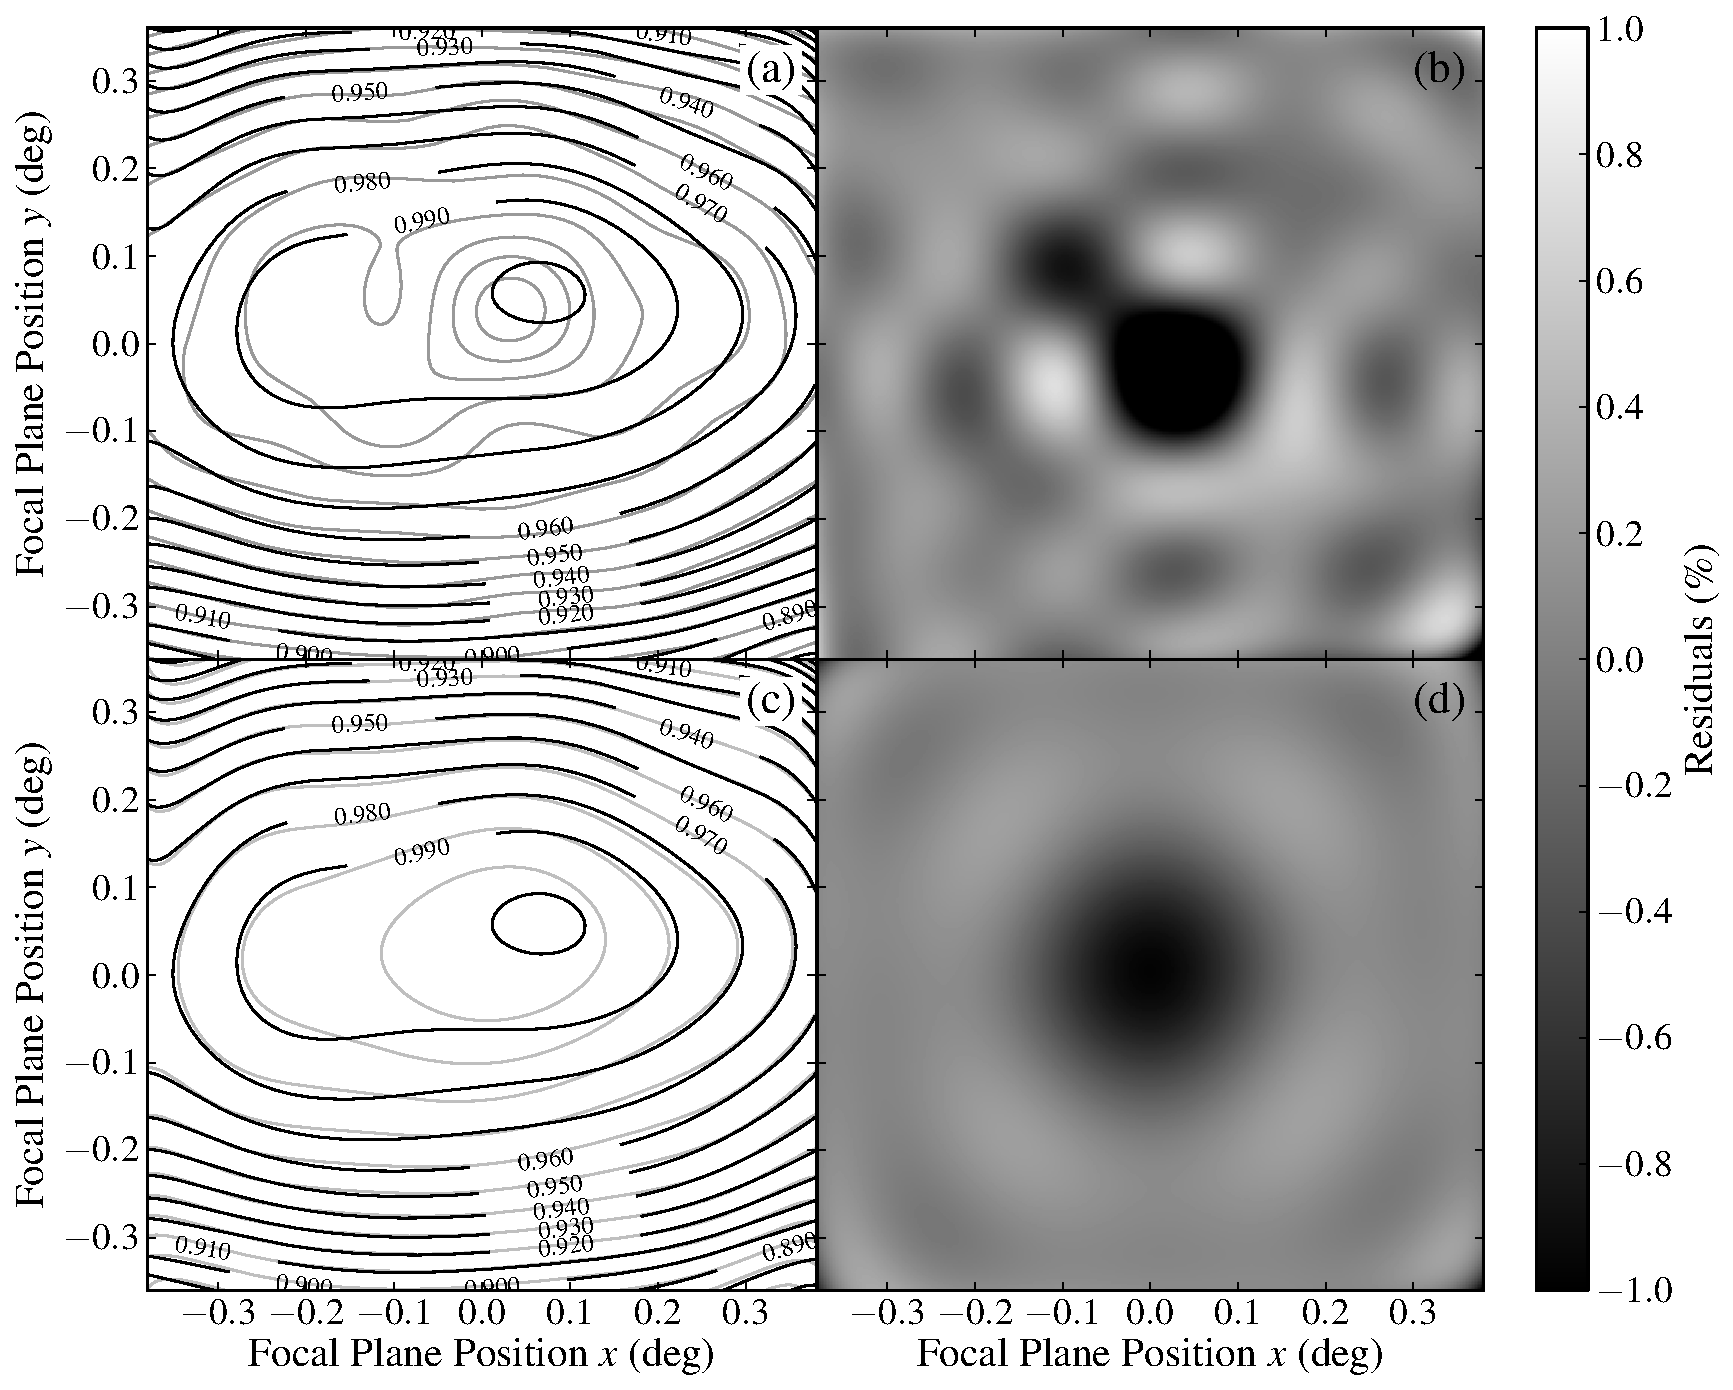
\includegraphics[width=\textwidth]{B_4160_ff.pdf}
\end{center}
\caption{A comparison of the fitted instrument response model $f_\fit(\vec{x_j} | \vec{q_\fit})$ obtained from self-calibrating the Survey B dataset compared to the true $f_\true(\vec{x} | \vec{q_\true})$ and best-in-basis $f_\basis(\vec{x_j} | \vec{q_\basis})$ instrument response models. The self-calibration procedure converged to the final solution after 4160 iterations. (a) Contour plot of the fitted (black) compared to the \textit{true} (gray) instrument response. (c) Contour plot of the fitted (black) compared to the \textit{best-in-basis} (gray) instrument response model. The best-in-basis instrument response is the best fit to the true instrument response possible with the basis used to model the instrument response in the self-calibration procedure (in this case an eighth order polynomial). The plots (b) and (d) show the residuals between the two instrument response models plotted in (a) and (c) respectively.\label{fig:B_result}}
\end{figure}

\begin{figure}[ht]
\begin{center}
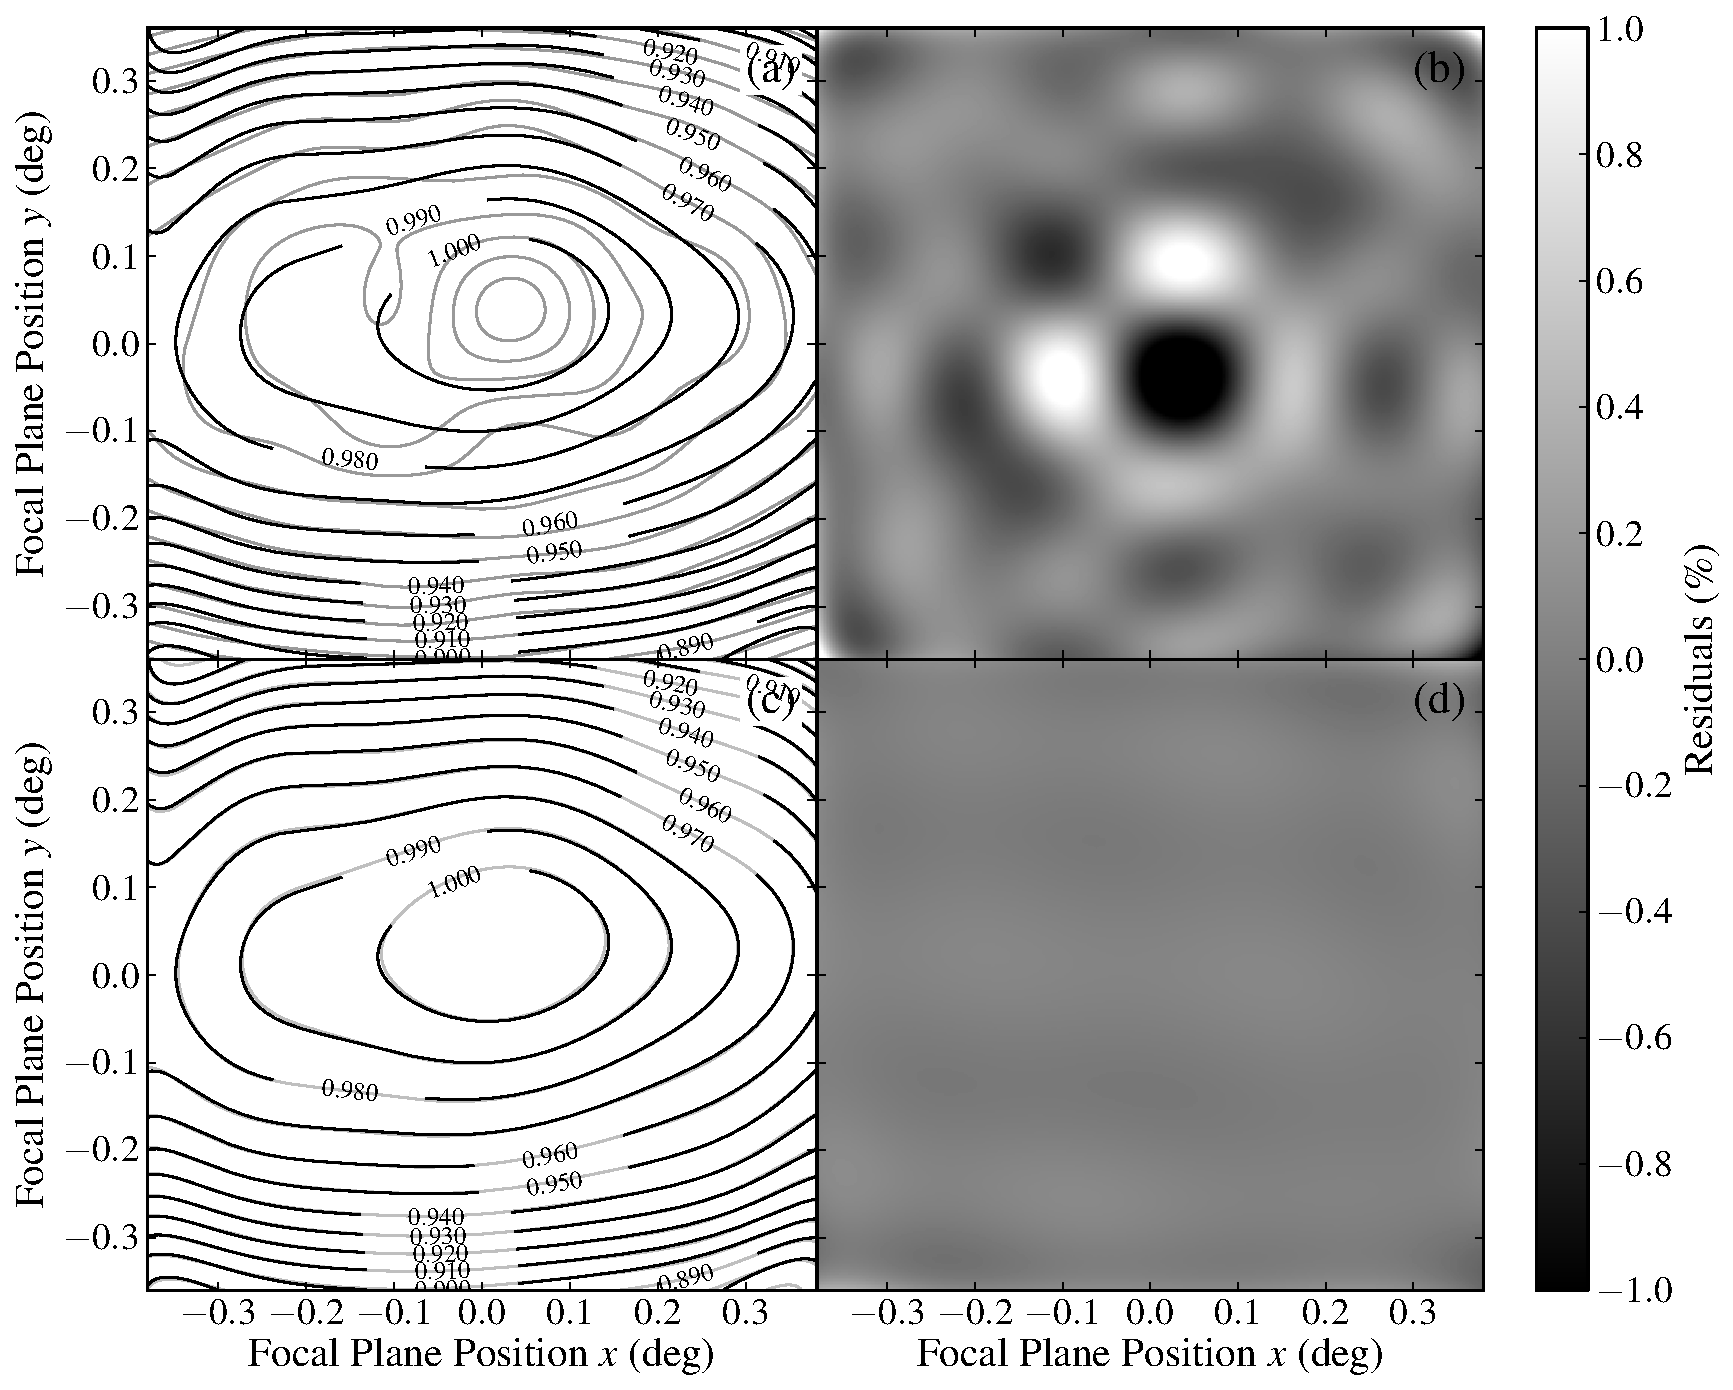
\includegraphics[width=\textwidth]{C_026_ff.pdf}
\end{center}
\caption{A comparison of the fitted instrument response model $f_\fit(\vec{x_j} | \vec{q_\fit})$ obtained from self-calibrating the Survey C dataset compared to the true $f_\true(\vec{x} | \vec{q_\true})$ and best-in-basis $f_\basis(\vec{x_j} | \vec{q_\basis})$ instrument response models. The self-calibration procedure converged to the final solution after 26 iterations. (a) Contour plot of the fitted (black) compared to the \textit{true} (gray) instrument response. (c) Contour plot of the fitted (black) compared to the \textit{best-in-basis} (gray) instrument response model. The best-in-basis instrument response is the best fit to the true instrument response possible with the basis used to model the instrument response in the self-calibration procedure (in this case an eighth order polynomial). The plots (b) and (d) show the residuals between the two instrument response models plotted in (a) and (c) respectively.\label{fig:C_result}}
\end{figure}

\begin{figure}[ht]
\begin{center}
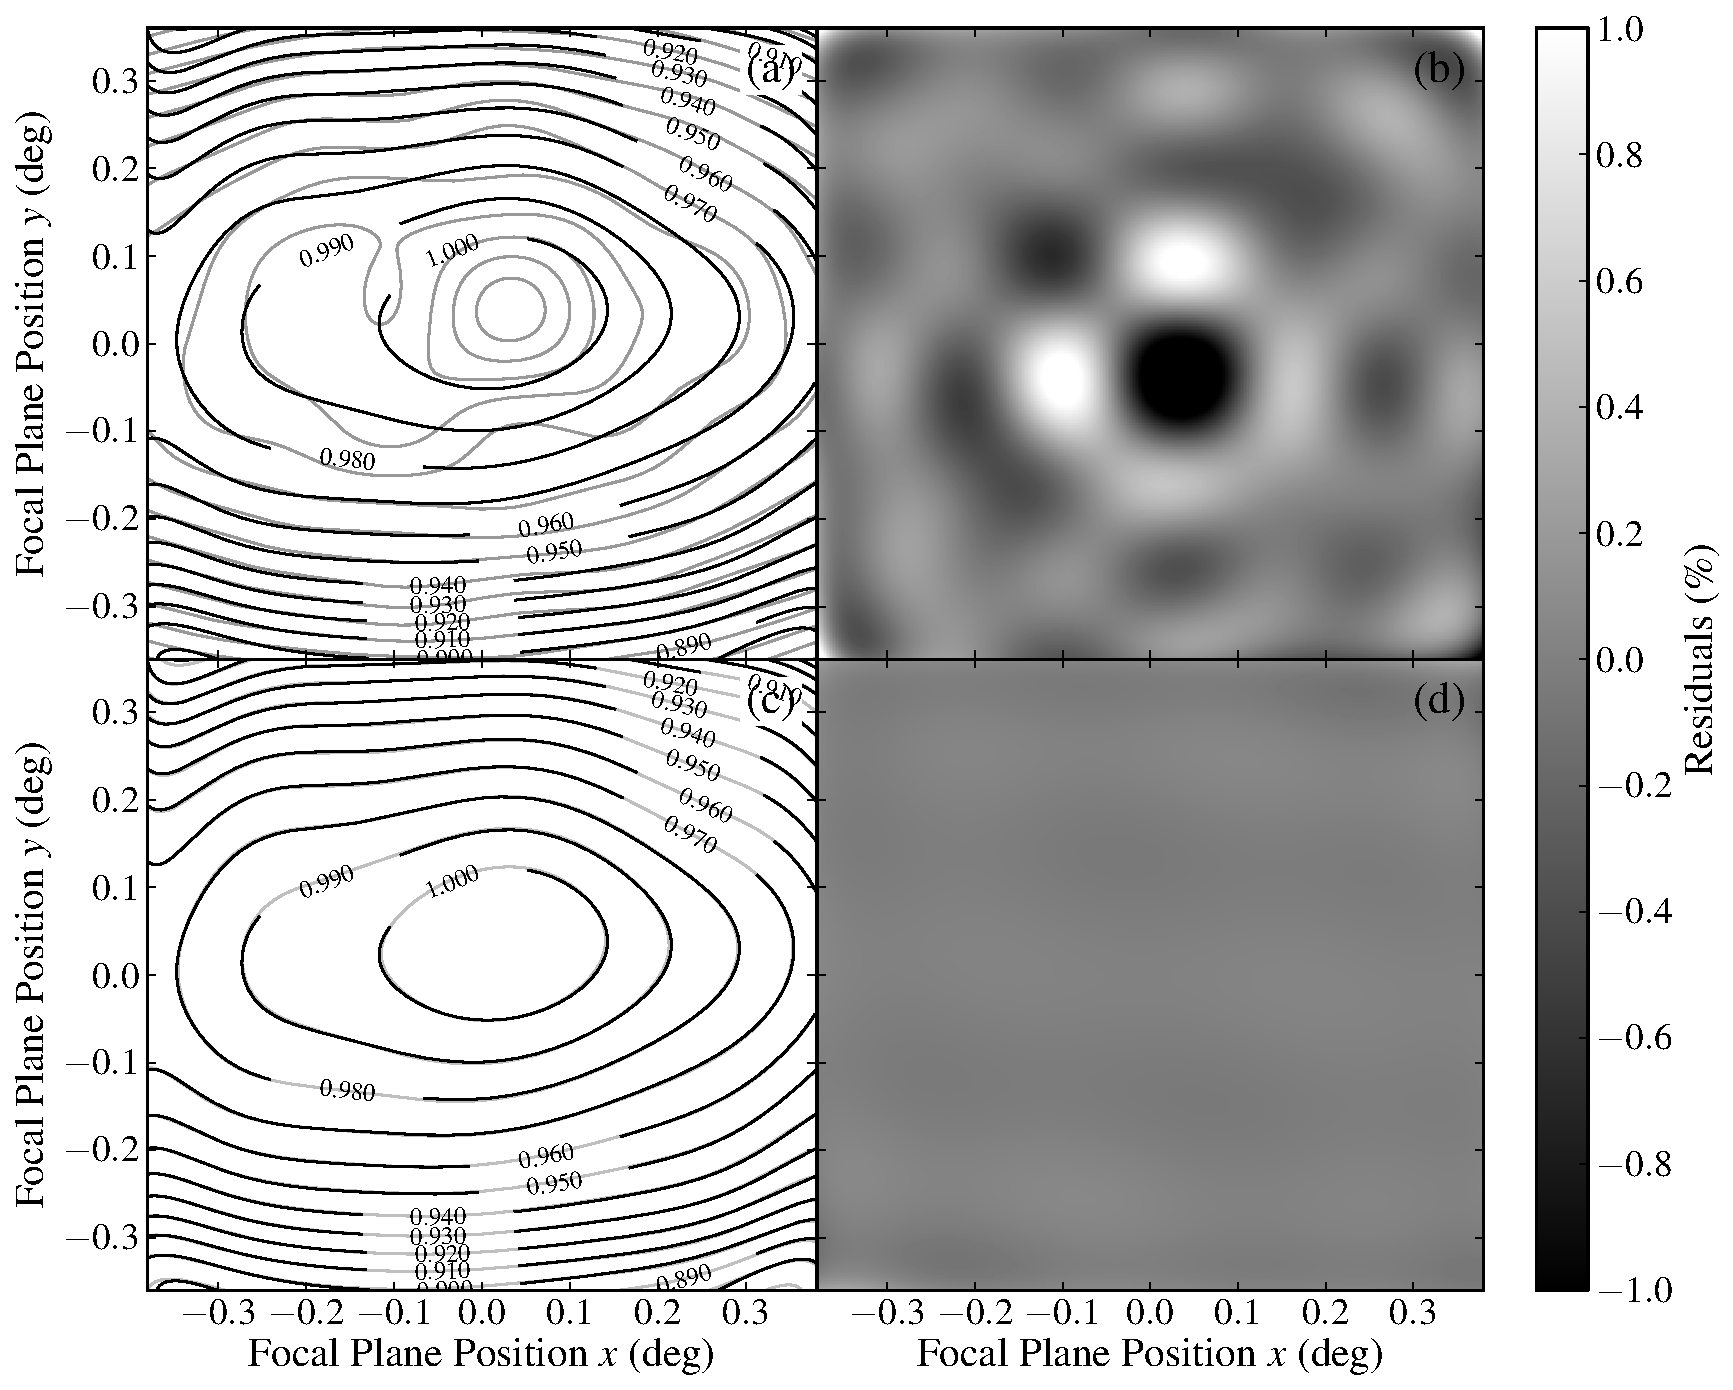
\includegraphics[width=\textwidth]{D_009_ff.pdf}
\end{center}
\caption{A comparison of the fitted instrument response model $f_\fit(\vec{x_j} | \vec{q_\fit})$ obtained from self-calibrating the Survey D dataset compared to the true $f_\true(\vec{x} | \vec{q_\true})$ and best-in-basis $f_\basis(\vec{x_j} | \vec{q_\basis})$ instrument response models. The self-calibration procedure converged to the final solution after 9 iterations. (a) Contour plot of the fitted (black) compared to the \textit{true} (gray) instrument response. (c) Contour plot of the fitted (black) compared to the \textit{best-in-basis} (gray) instrument response model. The best-in-basis instrument response is the best fit to the true instrument response possible with the basis used to model the instrument response in the self-calibration procedure (in this case an eighth order polynomial). The plots (b) and (d) show the residuals between the two instrument response models plotted in (a) and (c) respectively.\label{fig:D_result}}
\end{figure}

\clearpage
\begin{deluxetable}{ccccc}
\tablecaption{A summary of the quality of the final fit from the self-calibration procedure with the four simple survey strategies summarized in Table \ref{tab:simple_surveys}. The self-calibration procedure was run with only the brightest sources within the survey area; the source error $S_\text{RMS}$ corresponds to the measurements of these sources only and not all those within the survey. *Did not converge.\label{tab:simple_results}}
\tablehead{
\colhead{Survey Name} & \colhead{Iterations} & \colhead{Source Error $S_\rms$(\%)} & \colhead{True Badness $B_\true$ (\%)} & \colhead{Best-in-Basis Badness $B_\basis$ (\%)} }
\startdata
A*  & 8192 & 2.964 & 3.101 & 3.090 \\
B  & 4160 & 0.299 & 0.379 & 0.232 \\
C  & 26 & 0.199 & 0.305 & 0.043 \\
D  & 9 & 0.113 & 0.304 & 0.032 \\
\enddata
\end{deluxetable}

%% If you use the table environment, please indicate horizontal rules using
%% \tableline, not \hline.
%% Do not put multiple tabular environments within a single table.
%% The optional \label should appear inside the \caption command.

%% If the table is more than one page long, the width of the table can vary
%% from page to page when the default \tablewidth is used, as below.  The
%% individual table widths for each page will be written to the log file; a
%% maximum tablewidth for the table can be computed from these values.
%% The \tablewidth argument can then be reset and the file reprocessed, so
%% that the table is of uniform width throughout. Try getting the widths
%% from the log file and changing the \tablewidth parameter to see how
%% adjusting this value affects table formatting.

%% The \dataset{} macro has also been applied to a few of the objects to
%% show how many observations can be tagged in a table.

%% Tables may also be prepared as separate files. See the accompanying
%% sample file table.tex for an example of an external table file.
%% To include an external file in your main document, use the \input
%% command. Uncomment the line below to include table.tex in this
%% sample file. (Note that you will need to comment out the \documentclass,
%% \begin{document}, and \end{document} commands from table.tex if you want
%% to include it in this document.)

%% \input{table}

%% The following command ends your manuscript. LaTeX will ignore any text
%% that appears after it.

\end{document}

%%
%% End of file `sample.tex'.
